%-----------------------------------------------------------------------------
%
%               Template for sigplanconf LaTeX Class
%
% Name:         sigplanconf-template.tex
%
% Purpose:      A template for sigplanconf.cls, which is a LaTeX 2e class
%               file for SIGPLAN conference proceedings.
%
% Guide:        Refer to "Author's Guide to the ACM SIGPLAN Class,"
%               sigplanconf-guide.pdf
%
% Author:       Paul C. Anagnostopoulos
%               Windfall Software
%               978 371-2316
%               paul@windfall.com
%
% Created:      15 February 2005
%
%-----------------------------------------------------------------------------


\documentclass{sigplanconf}


% The following \documentclass options may be useful:

% preprint      Remove this option only once the paper is in final form.
% 10pt          To set in 10-point type instead of 9-point.
% 11pt          To set in 11-point type instead of 9-point.
% authoryear    To obtain author/year citation style instead of numeric.

\usepackage{amsmath}
\usepackage{graphicx}        % standard LaTeX graphics tool
\usepackage{subfigure}
\usepackage{epstopdf}
\usepackage{url}
\usepackage{algorithmic} 
\usepackage{algorithm2e}
\usepackage{amssymb}
\usepackage{amsmath}
\usepackage{fancybox}

\usepackage{subfigure}
\usepackage{fancyvrb}
\usepackage{listings}
\usepackage{color}
\usepackage{xcolor}
\usepackage[]{datetime}


\definecolor{dkgreen}{rgb}{0,0.6,0}
\definecolor{gray}{rgb}{0.5,0.5,0.5}
\definecolor{mauve}{rgb}{0.58,0,0.82}

\lstset{%frame=tb,
  language=Java,
  aboveskip=3mm,
  belowskip=3mm,
  showstringspaces=false,
  columns=flexible,
  basicstyle={\small\ttfamily},
  numbers= left,
	numbersep=6pt,
	numberstyle=\small,
  %frame=single,
  numberstyle=\tiny\color{gray},
  keywordstyle=\color{blue},
  commentstyle=\color{dkgreen},
  stringstyle=\color{mauve},
  breaklines=true,
  breakatwhitespace=true
  tabsize=2
	morecomment=[l]{//} 
	escapeinside={<@}{@>}
}
\begin{document}

\special{papersize=8.5in,11in}
\setlength{\pdfpageheight}{\paperheight}
\setlength{\pdfpagewidth}{\paperwidth}

\conferenceinfo{CONF 'yy}{Month d--d, 20yy, City, ST, Country} 
\copyrightyear{20yy} 
\copyrightdata{978-1-nnnn-nnnn-n/yy/mm} 
\doi{nnnnnnn.nnnnnnn}

% Uncomment one of the following two, if you are not going for the 
% traditional copyright transfer agreement.

%\exclusivelicense                % ACM gets exclusive license to publish, 
                                  % you retain copyright

%\permissiontopublish             % ACM gets nonexclusive license to publish
                                  % (paid open-access papers, 
                                  % short abstracts)

\titlebanner{banner above paper title}        % These are ignored unless
\preprintfooter{short description of paper}   % 'preprint' option specified.

\title{Program Repairing using Exception Types, Constraint Automata and Typestate}
%\subtitle{Subtitle Text, if any}

\authorinfo{Draft 4.0}
           {\today}
           {}
%\authorinfo{Name2\and Name3}
%           {Affiliation2/3}
%           {Email2/3}

\maketitle

\begin{abstract}

%marker
\textcolor{red}{\textbf{Changes done}}\newline

Runtime Exceptions are common types of exceptions which may lead to system crash which leads to shutdown or restart. 
For may critical application such scenario is unacceptable due to their nature which requires availability of the service. 
%Runtime exceptions may even leads to inconsistency of data in the system which may leads to further complications and expensive fixes.
Program bugs which causes runtime exceptions often go unnoticed at the time of development as these exceptions are unchecked exceptions. 
The key issue is to guide the program through some exception suppression procedure which will leads the program to a consistent state 
hence improve the chance of surviving a fatal crash. Here we consider such programs for which restart is not an option.

In this paper, we present a novel technique to recover from unexpected runtime exceptions.
 We have used hybrid of two techniques for efficient detection of potential point of failure and patch it closest to that to minimize the damage. 
 One technique uses type of runtime exception to apply appropriate patch.  
 The other technique will provides typestate analysis technique which will detect typestate violations to apply the right patch.
%The developer will flag a specific portion of the program to be eligible for repairing and patching.

\end{abstract}


%\category{CR-number}{subcategory}{third-level}

% general terms are not compulsory anymore, 
% you may leave them out
\terms
Reliability, Languages 

\keywords
program repair, runtime exception, software patching, symbolic execution, static analysis, type-state

\section{Introduction}
\label{sec:intro}

%marker
\textcolor{red}{\textbf{Changes done}}\newline

Exception handling attributes to the response of program during runtime to some exceptional condition encounter. 
Most of the time it changes normal flow of program. In many cases exception handling is natural part of software execution 
due to the nature of the software. 
An application which constantly accesses I/O which also includes share resources may throw exception if another application blocks it. 
Here in this paper we discuss and analyze java exceptions and produce repair patch based on that. Java supports two types of exceptions : 
\begin{itemize}
	
	\item \textbf{Checked exception} which requires explicit \emph{throws} declaration at the method declaration or \emph{try-catch} 
	block by the developers. Such exceptions are handled carefully as they often involves accessing resources like network, database, 
	file system, I/O etc. 
	
	\item \textbf{Unchecked exception} which does not enforce similar handing mechanism as the former one. \emph{java.lang.RuntimeException} 
	and its subclasses and \emph{java.lang.Error} are types of unchecked exceptions. \emph{NullPointerException}, \emph{ArrayIndexOutOfBound}, 
	\emph{ArithmeticException} are examples of common java runtime exceptions.

\end{itemize}

Oracle official documentation says that ``\emph{Here's the bottom line guideline: If a client can reasonably be expected to recover from an exception,
 make it a checked exception. If a client cannot do anything to recover from the exception, make it an unchecked exception}".  
 Unchecked exception, particularly runtime exceptions can be thrown from any point in the program making them quite unpredictable in nature. 
 Due to this extensive testing phase is required to eliminate any bugs and solve corner cases. 
 Yet many applications suffer unexpected runtime exception causing system crash which leads to shutdown or restart.

We find out many applications where system shutdown/restart is expensive due to their nature. 
Notable examples are air traffic control, auto pilot, life support system, smart power grids, telephone networks, 
robots like UAV and rovers deployed for surveillance, reconnaissance and knowledge acquisition in remote locations etc. 
These applications are real-time sensitive and there is no room for exception handling in such system. 
Sudden crash involves risk of human life, expensive equipments and critical services. 
Other example includes web applications which uses scrips to dynamically generate websites and interfaces as per customer preferences. 
Many E-commerce websites handles queries, access and process customer and shopping items data and commits large amount of transactions. 
Sudden system crash may result in loss of precious time and data which eventually may result in a frustrated customers move to other websites. 
Many time bad or malicious code leads to some vulnerability to critical applications and website which can be exploited by attack to orchestrate 
system crash. Thought these examples cover a large variety of applications, all of them point to some concern of \emph{availability}.

Usually, developers tests their code in series of verifications which involves code review, static and dynamic analysis of the code, 
generate test cases to cover as much potential input .Yet may corner cases can be left overlooked which can cause runtime exceptions. 
Multi-threaded applications are also susceptible to erroneous thread interleaving. One such exception is \emph{java.lang.IllegalMonitorStateException},
 when a thread has attempted to wait on an object's monitor or to notify other threads waiting on an object's monitor 
 without owning the specified monitor.Applications under adversarial situation should be considered where deliberate malicious input may cause it to fail. 
 To recover from such situation, a mechanism is needed which can predict failure by doing invariant and symbolic analysis. 
 Invariant analysis will detect particular variables outside legal/safe bound. Symbolic analysis will indicate to the potential point of failure. 

In this paper we proposed two solution to suppress runtime example and ensure system survivability. The approach consists of four primary phases

\begin{itemize}
	\item \textbf{Generate input data-set} : We index user input along with the global variables and method arguments of successful runs. 
	The local variables are not indexed as they can be re-generated. 
	These data-set is used as a reference to later executions which encounters runtime exceptions. 
	Appropriate user input of previous successful run is chosen in terms of correlation coefficient. 
	
	\item \textbf{Program slice for patching} : We perform static analysis prior to running the program to determine data dependencies of the variables. 
	The analysis yields a dependency graph which is used to determine optimal slice to be used as patch. 
	This patch is placed in catch block and executed with the values of previous successful run while the original code is wrapped in try block.
	
	\item \textbf{Determine type of exception and patching} : The characteristics of patching is dependent on the type of runtime exception 
	encountered by the program. A piece of code may throws multiple types of exceptions and all of them are handled at the time of patching by 
	instrumenting multiple catch blocks.
	
	\item \textbf{Use typestate for repairing} : Typestate analysis, sometimes called protocol analysis defines valid sequences of operations 
	that can be typically modeled using Finite State Machine (FSM) where the states represent abstract state of the program and the symbols are 
	certain method invocations to perform state transition. Typestates are capable of representing behavioral type refinements like Iterators, 
	where \emph{hasNext()} method should be called before the \emph{next()} method call. 
	Typestate analysis is widely used as a safety feature to ensure a certain sequence of operations maintains proper protocol or not. 
%But this method is unconventional and investigated in the field of program repairing.
The documentations of the API used in the application will define the valid typestate for repairing.
\end{itemize}

The object of the patching is to repair the problem closest to it to minimize any collateral damage to other parts of the applications hence minimizing the chance of unintentional data loss/corruption. 

\section{Motivation and Challenges}
\label{sec:mot}

\subsection{Data from Stack overflow posts}
\label{subsec:stackoverflow}

\begin{table}[h]
\caption{Most frequent java rumtime exceptions from stack overflow data}
\label{tab:stackoverlow}
\begin{tabular}{|c|c|c|}
\hline
\textbf{Runtime Exception Type} & \textbf{Occurrences} & \textbf{Percentage}\\
\hline NullPointerException & $34912$ & $54.94\%$ \\ \hline

ClassCastException & $7504$ & $11.81\%$ \\ \hline

IndexOutOfBoundsException & $6637$ & $10.44\%$ \\ \hline

SecurityException  & $5818$ & $9.15\%$ \\  \hline

NoSuchElementException & $2392$ & $3.76\%$ \\ \hline

ArithmeticException & $2338$ & $3.67\%$ \\ \hline

ConcurrentModificationExceptio & $1889$ & $2.97\%$ \\ \hline

DOMException & $1024$ & $1.61\%$ \\ \hline

ArrayStoreException & $279$ & $0.43\%$ \\ \hline

MissingResourceException & $277$ & $0.43\%$ \\ \hline

BufferOverFlowException & $161$ & $0.25\%$ \\ \hline

NegativeArraySizeException & $122$ & $0.19\%$ \\ \hline

BufferUnderFlowException & $66$ & $0.1\%$ \\ \hline

LSException & $64$ &  $0.1\%$ \\ \hline

MalformedParameterizedTypeExce & $38$ & $0.05\%$ \\ \hline

CMMException  & $8$ & $0.01\%$ \\ \hline

FileSystemNotFoundException & $6$ & $0.009\%$ \\ \hline

NoSuchMechanismException & $3$ & $0.0045\%$ \\ \hline

MirroredTypesException & $1$ & $0.0015\%$ \\ \hline

\end{tabular}
\end{table}



We have analyzed data from stack overflow. From the stack overflow data dump, we
look for java runtime exception which are discussed most frequently. In the
table~\ref{tab:stackoverlow}, the dta we find is tabulated along with their
occurrences and percentages.



%marker
%\textcolor{red}{\textbf{To Do}}\newline


\section{Problem Formulation}
\label{sec:form}

\textcolor{red}{\textbf{This part is incomplete, I am now writing the strategy part}}\newline
We formulate the problem in following way

\subsection{Runtime Exceptions}
\label{subsec:excep}

\begin{figure}[!htb]
\centering
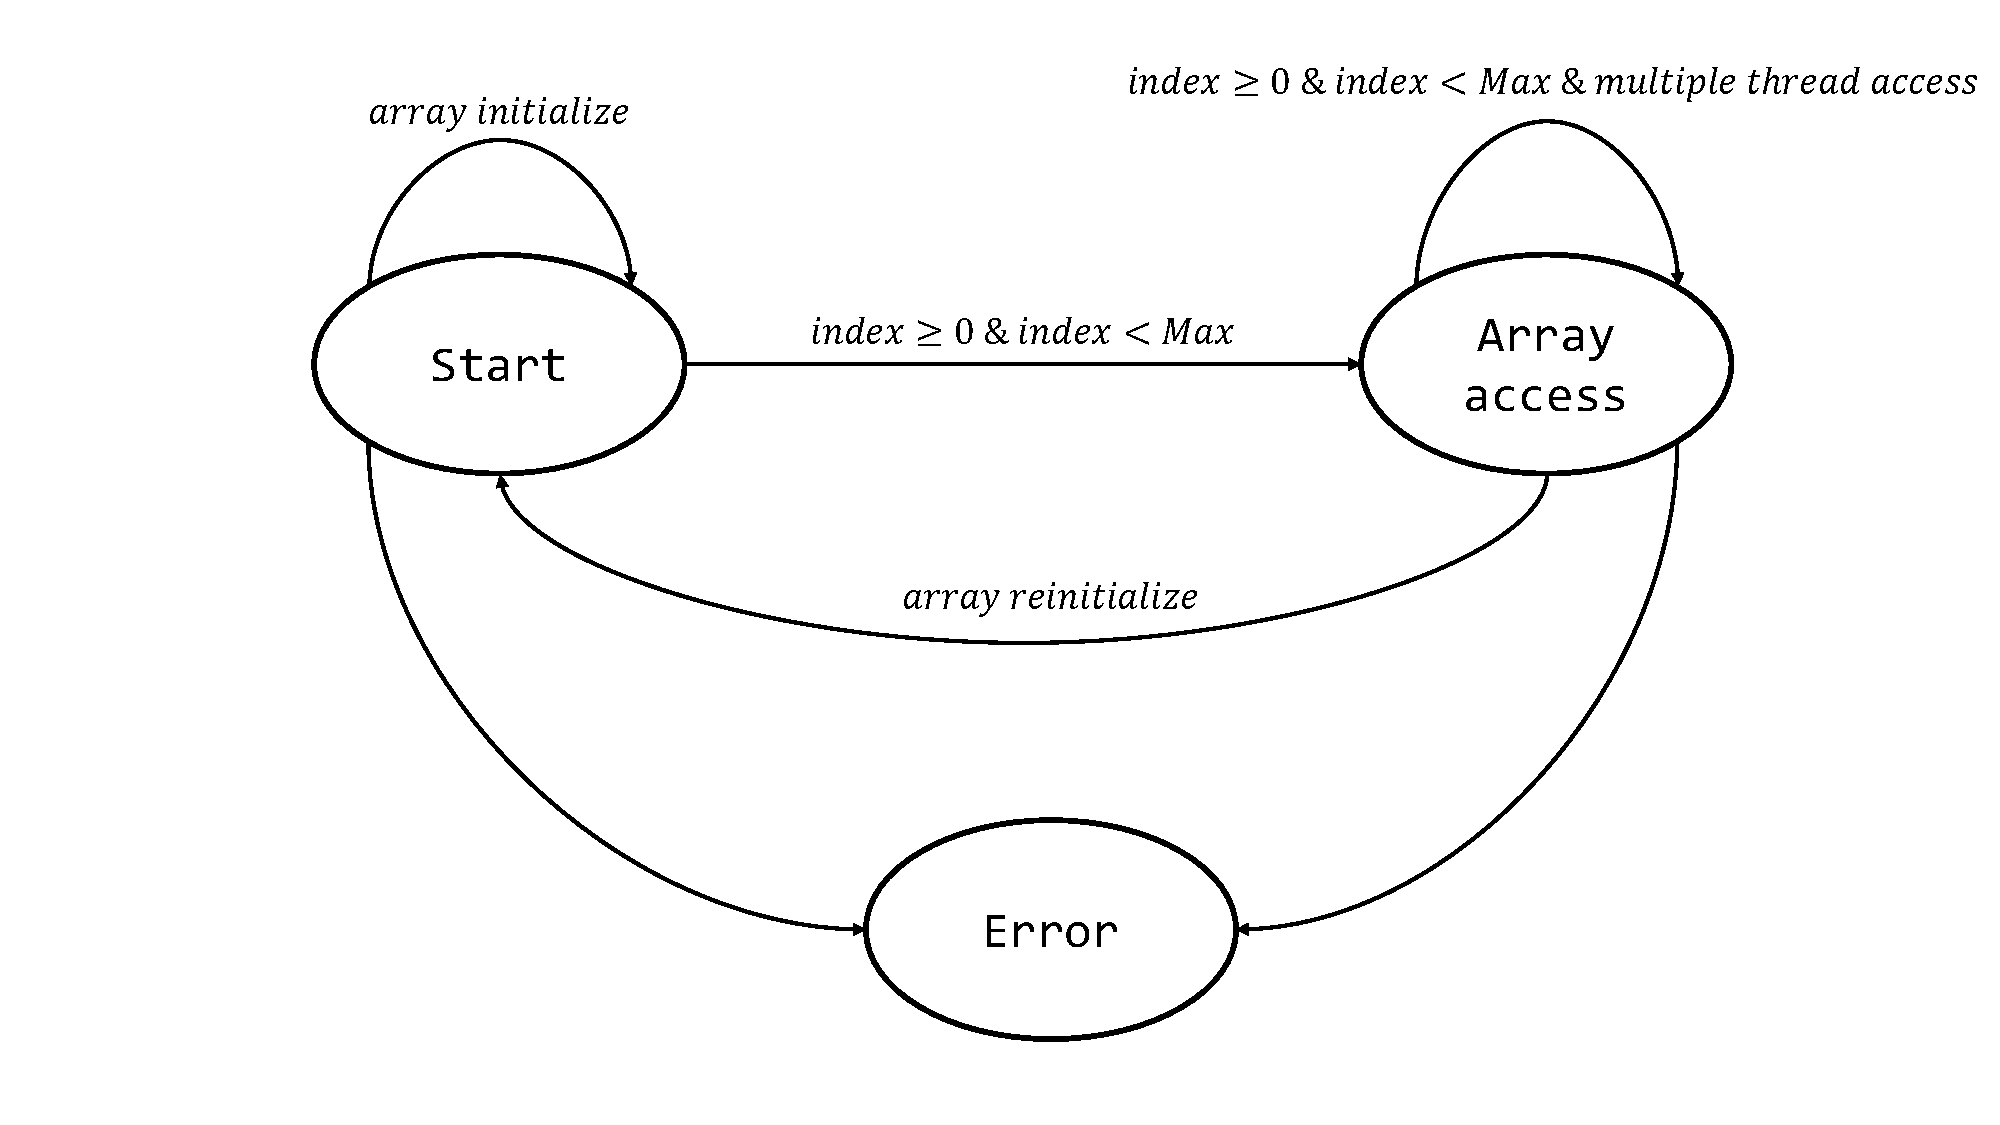
\includegraphics[width=3.2in]{images/ArrayIndex.pdf}
\caption{array index out of bound formulated as FSM}
\label{fig:array}
\end{figure}


We can visualize all runtime exceptions as finite state machine (FSM). When a program violates such sequence, it throws runtime exception. 
In Figure~\ref{fig:array}, array index out of bound (java.lang. ArrayIndexOutOfBoundException) exception is described as a FSM. 
Here, a program will be in safe bound as long as the $array\_index \geq 0$ or $array\_index \leq max\_array\_size - 1$


\section{Repairing Strategy:Exception Type}
\label{sec:strgEx}

%marker
\textcolor{red}{\textbf{Please review this section}}\newline


\lstset{language=Java, caption=Java code which may throws runtime exceptions, label=example1}
\begin{lstlisting}

public class TestClass
{
	private int[] arr1;
	private int[] arr2;
	private int[] arr3;
		
	public TestClass(int[] arr1, int[] arr2, int[] arr3)
	{
		this.arr1 = arr1;
		this.arr2 = arr2;
		this.arr3 = arr3;
	}
	public int[] fun(int a, int b, int c, int d)
	{
		int temp0 = a + b;
		int temp1 = c * d;
		int temp2 = temp0 - temp1;
		//array index out of bound, negative index
		int temp3 = this.arr1[temp0];
		//array index out of bound, negative index
		int temp4 = this.arr2[temp1];
		//array index out of bound, negative index
		int temp5 = this.arr3[temp3];
		int temp6 = temp4 + temp5;
		int temp7 = temp6 - temp3;
		//array index out of bound, negative index, divide by zero
		this.arr1[temp6] = temp7/(d-a);
		//array index out of bound, negative index, divide by zero
		this.arr2[temp7] = temp7/temp4;
		if(arr2[temp1] ! = arr3[temp7])
			return arr1;
		else
			return null;
	}
}
public class MainClass 
{
	public void main(String[] a) 
	{
		int[] arr1 = {1,2,3,4};
		int[] arr2 = {1,2,3,4};
		int[] arr3 = {1,2,3,4};
		TestClass TC = new TestClass(arr1, arr2, arr3);
		int[] res = TC.fun(2,4,3,4);
		//Null pointer exception
		System.out.print("Result : "+res[2]);
	}    
}
\end{lstlisting}

In the Example~\ref{example1}, we have given a piece of java code which shows multiple lines can throw several runtime exceptions. 
In this example we consider three very common runtime exceptions: NullPointerException, ArrayIndexOutOfBoundExcepltion, NegetiveIndexException, 
ArithmeticException (i.e. divide-by-zero). In rest of this section, this particular example will be used to demonstrate the repairing strategy.

\subsection{Symbolic Analysis}
\label{subsec:symb}


\begin{figure}[!htb]
\centering
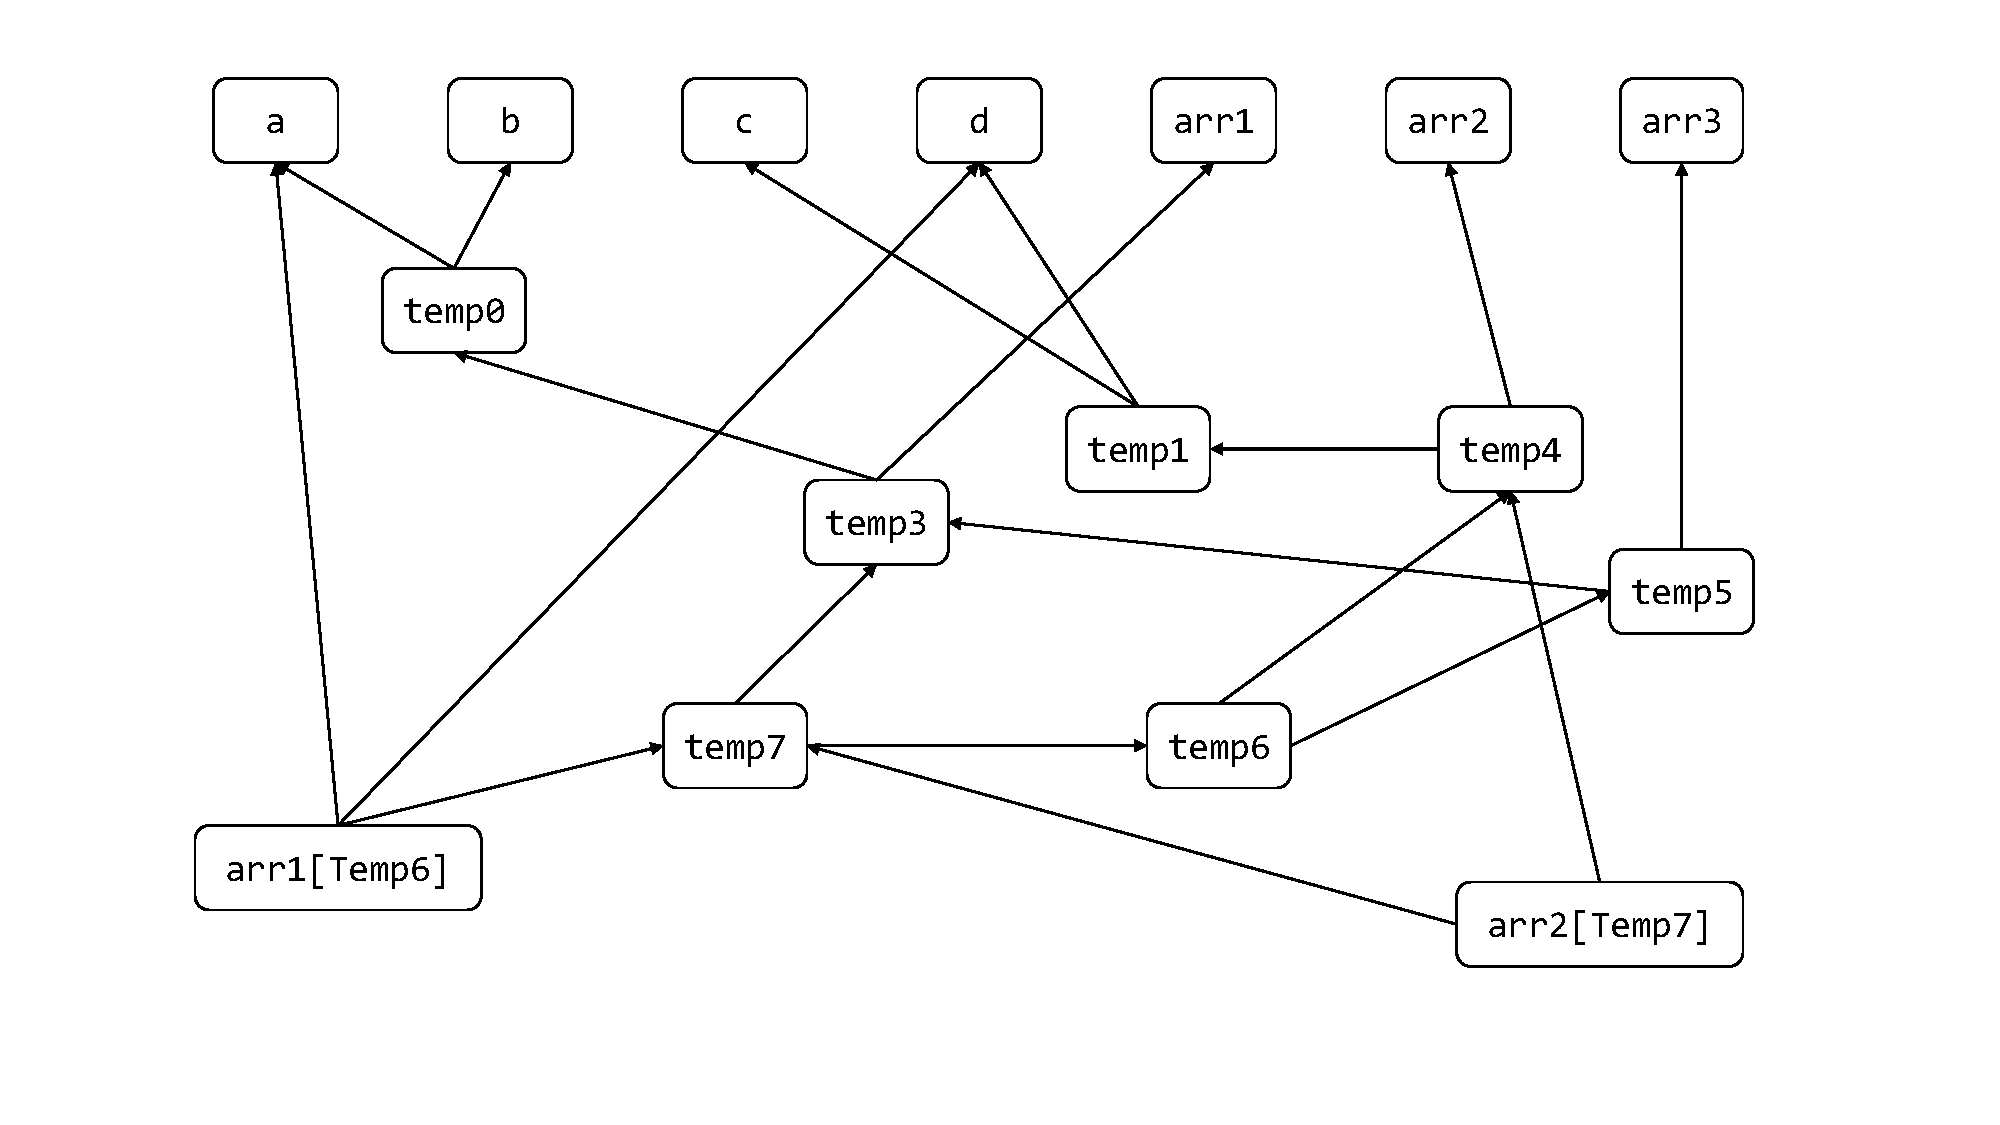
\includegraphics[width=3.3in]{images/depG.pdf}
\caption{Data dependency graph of the variables in Example\ref{example1}}
\label{fig:datadep}
\end{figure}

We have done several  static analysis a priori  over the Java source code to discover :
\begin{enumerate}
	\item Critical section of the code which are not eligible for patching. Eg. banking or any financial transaction which should be crashed in case of 
	exception as suboptimal solution due to patching will led it to inconsistent state.
	\item Symbolic analysis of the program to discover potential points of failure and mark them.
	\item Build data dependency graph which will be used to generate appropriate code slice to be used as patch. 
	In Figure~\ref{fig:datadep}, the data dependency graph of the example code~\ref{example1} is presented.
	\item The symbolic analysis will also reveal which kind of exception is likely to happened at the time of execution. 
	This information is necessary at the time of instrumenting the patch as it will determine the catch block.
	
\end{enumerate}

\subsection{Data set for Successful Program Runs}
\label{subsec:progrun}

Here we will store all the traces of successful program runs.
\begin{figure}[!htb]
\centering
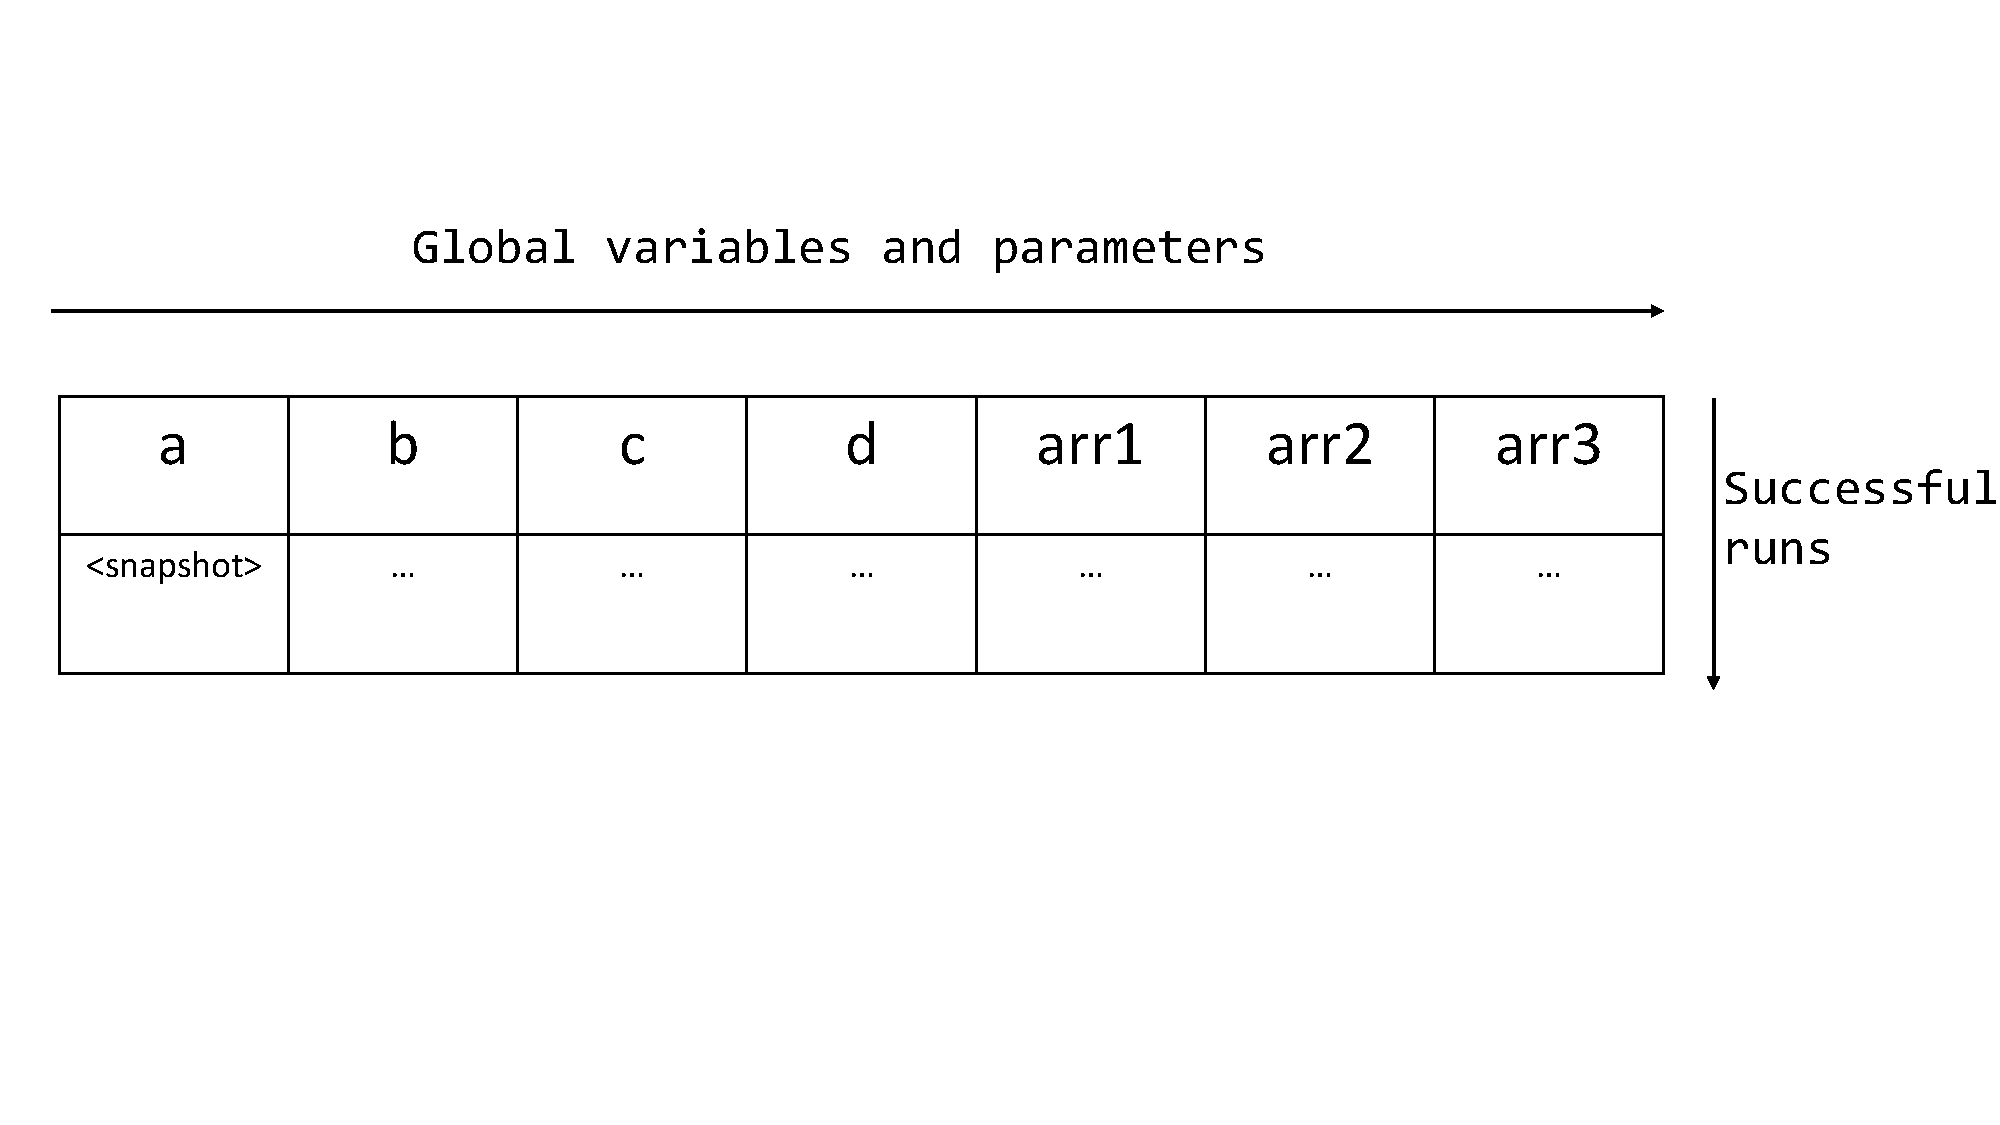
\includegraphics[width=3.0in]{images/succrun.pdf}
\caption{Indexed global variables and method arguments successful runs}
\label{fig:succrun}
\end{figure}

Figure~\ref{fig:succrun} shows such indexed traces of all the global variables and method arguments. 
We store the snapshots of these objects. We won't store local variables as they can always be regenerated. 
As it is required to capture the snapshot of all these variable, we made deep cone of all of these objects and variables. 

%begin{table}[htb]
%\begin{tabular}{|c|c|c|c|c|c|c|}
%\hline
%a & b & c & d & arr1 & arr2 & arr3 \\ \hline
%\ldots & \ldots & \ldots & \ldots &	\ldots & \ldots & \ldots\\ \hline
%\end{tabular}
%\caption{Trace of successful runs}
%	\label{tab:Trace}
%\end{table}


\subsection{Matrices}
\label{subsec:martices}

%marker
\textcolor{red}{\textbf{Please review this section.}}\newline

\subsection{Instrumenting Patching}
\label{subsec:patchinstru}

We have used Soot framework which is a Java byte code manipulator to instrument patch. 
The patching technique is divided into two phases

\subsubsection{Determine Exception Type} 

At the time of execution, the exception may happened due to some specific values of some variables. We will catch the exception. Here the type of 
runtime exception is $java.lang.ArrayIndexOutOfBound$. This will be used to produce the try-catch block.
 
\subsubsection{Determine Optimal Code Slice}

The optimal code slice will be determined from the data dependency graph which was rendered at the time of static analysis mentioned in 
Section~\ref{subsec:symb}. In the Listing~\ref{patchingexample1}, the example code snippet shows such code slice inside the catch block. 
As the error occurred at the line $int\ temp5\ =\ this.arr3[temp3];$ the statements which produces the temp3 and the statement which also 
involves $temp3$ or any other variables derived from $temp3$, would be included in the catch block for re-execution with the valued of the 
same from the data table of previous successful runs.

 

\lstset{language=Java, caption=patching code slice based on exception type, label=patchingexample1}

\begin{lstlisting}

public class TestClass
{
	private int[] arr1;
	private int[] arr2;
	private int[] arr3;
		
	public TestClass(int[] arr1, int[] arr2, int[] arr3)
	{
		this.arr1 = arr1;
		this.arr2 = arr2;
		this.arr3 = arr3;
	}
	public int[] fun(int a, int b, int c, int d)
	{
		try
		{
		  int temp0 = a + b;
		  int temp1 = c * d;
		  int temp2 = temp0 - temp1;
		  int temp3 = this.arr1[temp0];
		  int temp4 = this.arr2[temp1];
	   //IndexOutOfBoundException as temp3 = 20
		  int temp5 = this.arr3[temp3];
		  int temp6 = temp4 + temp5;
		  int temp7 = temp6 - temp3;
		  this.arr1[temp6] = temp7/(d-a);
		  this.arr2[temp7] = temp7/temp4;
		}
		catch(IndexOutOfBoundsException indEx)
		{
		  int temp0 = a + b;
		  int temp1 = c * d;
		  int temp2 = temp0 - temp1;
		  int temp3 = this.arr1[temp0];
		//Bellow line is not part of the patch as 
		//temp1 and temp3are not related to temp3 
		//for which the exception occurred.
		  //int temp4 = this.arr2[temp1];
		  int temp5 = this.arr3[temp3];
		}
		if(arr2[temp1] ! = arr3[temp7])
			return arr1;
		else
			return null;
	}
}
public class MainClass 
{
	public void main(String[] a) 
	{
		int[] arr1 = {20,21,22,23};
		int[] arr2 = {1,2,3,4};
		int[] arr3 = {10,11,12,13};
		TestClass TC = new TestClass(arr1, arr2, arr3);
		int[] res = TC.fun(2,4,3,2);
		System.out.print("Result : "+res[2]);
	}    
}
\end{lstlisting}

\subsection{Variable Tracking and Monitoring}
\label{subsec:taint}
\textcolor{red}{\textbf{I have added standard taint analysis technique here as an example. We can change it later}}\newline


Here we used taint analysis technique to tag variables and objects of our interest to monitor them. 
This steps are necessary as the values of the variables used during the instrumentation may cause further runtime exceptions. 
We used bit-vector which is an efficient technique to taint a object/variable. 
It requires maintain a single dimension byte array where each bit correspond to a single object/variable of our interest. 
The bit values will be flipped when it is required to taint ($1$) or untaint ($1$) an object/variable. 
We will only monitor these entities until all of them flushed from the program and the entire program reached to a stable state.

\section{Repairing Strategy : Constraint Automata}
\label{sec:strgCA}

\subsection{General Structure}
\label{subsec:generalCA}

\emph{Constraint automata} is a formalism to describe the behavior and possible data flow in coordination models. 
Mostly used for model checking. We have used it for the purpose of program repairing technique. Here we define the finite state automata as follows :

$$(Q, \Sigma, \delta, q_0, F)$$
\begin{itemize}
	\item $Q$: set of state where $|Q| = 2$, \emph{legal state}(init) and \emph{illegal state} (error).
	\item $\Sigma$: symbols, invariants based on exception type.
	\item $\delta$: transition function. $init \rightarrow init$ is safe transition and $init \rightarrow error$ is the invariant violation.
	\item $q_0$: starting state, here $q_0 = init$.
	\item $F$: end state, here it same as $q_0$.
\end{itemize}

\begin{figure}[!htb]
\centering
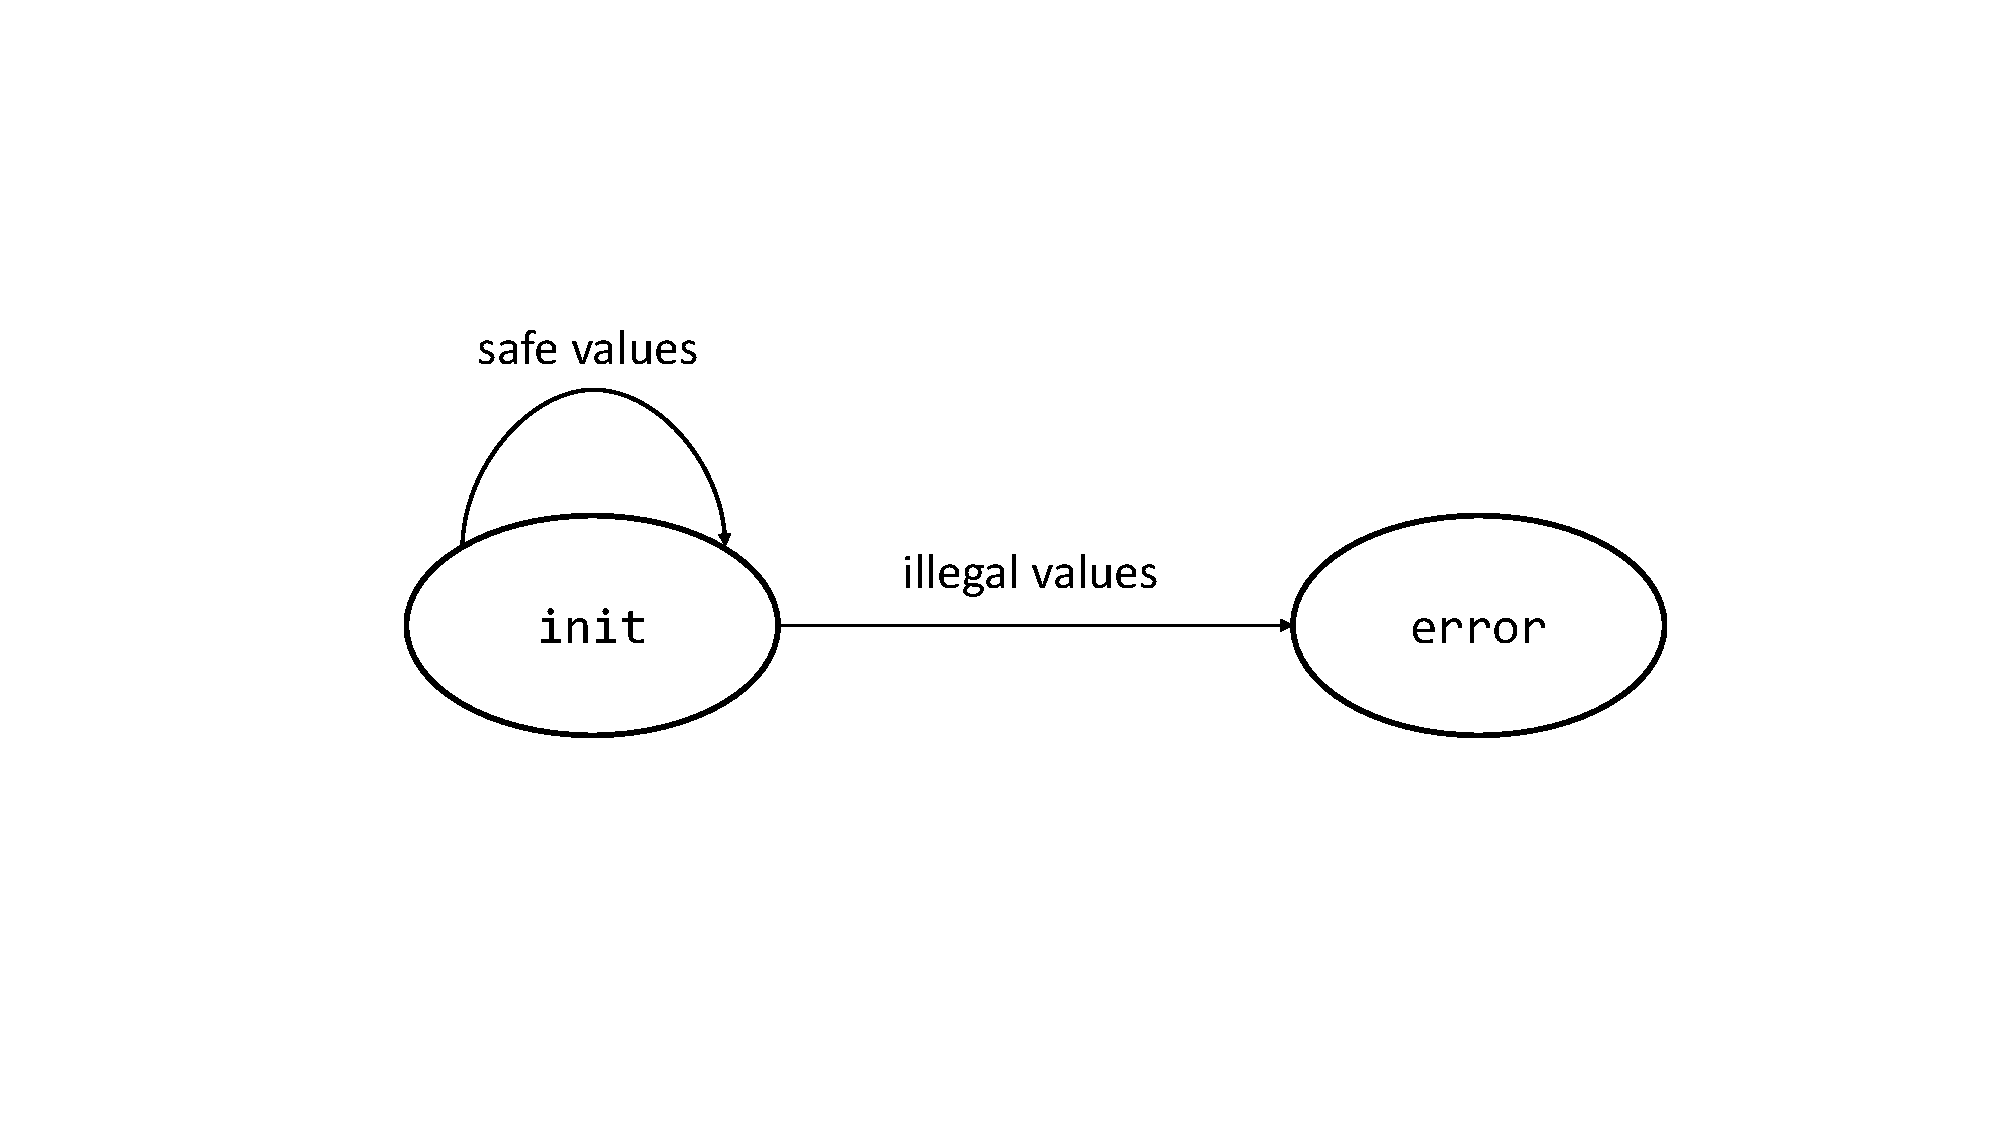
\includegraphics[width=3.2in]{images/automata.pdf}
\caption{Constraint automata general model}
\label{fig:automata}
\end{figure}

According to the Figure~\ref{fig:automata}, the repairing mechanism will only trigger when we have a transition from 
init state to error state due to invariant violation.

\subsection{Patching Techniques}
\label{subsec:patchCA}

The patching technique is based on the exception type. 

\subsubsection{Array index out of bound exception}

Array index out of bound exception happen when one tries to access the array with a index which is more than the size of the array or 
less than zero i.e. with some negative value. We did the patching based on these two scenario. When the index is more than the array size, 
we patch it by assigning $array.length - 1$.

\lstset{language=Java, caption=array index out of bound patching, label=patchingexample2}

\begin{lstlisting}
void foo()
{
  int []arr = {1,2,3,4};
  int index = 10;
  int y = 0;
  try
  {
    //original code
    y = arr[index];
  }
  //patching instrumentation
  catch(IndexOutOfBoundException ex)
  {
    if(index > arr.length)
      y = arr[arr.length - 1];
    else
      y = a[0];
  }
}

\end{lstlisting}

\subsubsection{Negative Array Size Exception}

Negative array size exception occurs when one tries to create a array with a negative size. 
The patching is done based on data flow analysis. Suitable index size is determined by looking at the successive statement dependent on the array. 
To take a safe bound, we took maximum index size and set as the array size in the new array statement.


\lstset{language=Java, caption=arr index out of bound patching, label=patchingexample2}

\begin{lstlisting}
void foo()
{
  int []arr = {1,2,3,4};
  int index = 10;
  int y = 0;
  try
  {
    //original code
    y = arr[index];
  }
  //patching instrumentation
  catch(IndexOutOfBoundException ex)
  {
    if(index > arr.length)
      y = arr[arr.length - 1];
    else
      y = a[0];
  }
}

\end{lstlisting}

\subsubsection{Arithmetic Exception : Division-by-zero Exception}

Division by zero causes arithmetic exception. There are two different cases which were considered here. 
\begin{itemize}
	\item \textbf{Case I :} The denominator is going to the taint sink but the left hand side is not going to any taint sink. 
	Here we will not manipulate the denominator as we are not manipulating any variable which are going to any taint sink.
	\item \textbf{Case II :} The denominator and the left hand side, both are not going to any taint sink. So they are safe to patch.
\end{itemize}

\lstset{language=Java, caption=arithmetic exception : division-by-zero patching, label=patchingexample2}

\begin{lstlisting}
void foo()
{
  int a = 10;
  int b = 0;
	int y;
  try
  {
    //original code
    y = a/b;
  }
  //patching instrumentation
  catch(ArithmeticException ex)
  {
    //case I
    if(taintSink(b))
      y = 0;
    //case II
    else
    {
      b = 1;
      y = a/b;
    }
  }
}
\end{lstlisting}

\subsubsection{Null Pointer Exception}

Null pointer exception in Java is the most common runtime exception encountered. 
Thrown when an application attempts to use null in a case where an object is
required. There exists various scenarios where null pointer exception can
happen. These different scenario requires different patching techniques. Bellow
we enlist all cases and corresponding patching techniques.


\begin{itemize}
  \item \textbf{Case I} Calling the instance method of a null object. \newline
  \textbf{Patch :} This is patched by calling the constructor. In case there
  exists more than one constructor then we need to find most appropriate
  constructor. This is done by using data flow analysis in the successive
  statement to see which fields/methods been accessed and according to that
  most suitable constructor should be picked up, this will ensure safest way to
  deal with the later method calls/field accesses.
  
  \lstset{language=Java, caption=appropriate constructor, label=patchingexample2}

\begin{lstlisting}
class MyClass
{
 Integer field1;
 String field2;
 Double field3;

 public MyClass()
 {
  this.field1 = 1;
  this.field2 = null;
  this.field3 = null;
 } 
 public MyClass(Integer field1, String field2)
 {
  this.field1 = field1;
  this.field2 = field2;
  this.field3 = null;
 } 
 public MyClass(Integer field1, String field2, Double field3)
 {
  this.field1 = field1;
  this.field2 = field2;
  this.field3 = field3;
 }
 public Double getfield3()
 {
  return this.field3;
 }
}

class main
{
 Myclass mclass = null;
 Double a = null;
 try
 {
  //original code
  a = mclass.getfiled3() + 5.0;
 }
 //instrumentation
 catch(NullPointerException ex)
 {
  //choose appropriate constructor
  mlass = new MyClass(1, "a", 1.0); 
  a = mclass.getfiled3();
 }
}
\end{lstlisting}
  \item 
  
  \item \textbf{Case II} Possible Accessing or modifying the field of a null
  object.\newline
  \textbf{Patch :} The patch is same as the previous one.
  
  \item \textbf{Case III} Taking the length of null as if it were an
  array.\newline
  \textbf{Patch :}The patch for this situation is very much similar to the
  negative array size exception. Here we will do a data-flow analysis to see all
  the successive statements where the array object has been used (read or
  write). For safety we will take the maximum index from those statements and
  reinitialize the array object with the size.
    
  \lstset{language=Java, caption=array null pointer exception,
  label=patchingexample2}

\begin{lstlisting}
int[] bar(int a)
{
 int []arr = new int[a];
 int []b = (a > 10) ? arr:null;
 return b; 
}
void foo()
{
 int[] arr;
 int []arr = bar(5);
 try
 {
  //access or modify any field of arr
  //this will throw a null pointer exception
 }
 //instrumented code
 catch
 {
  int ARRAY_SIZE = 11;
  int []arr = new int[ARRAY_SIZE];
  //access or modify any field of arr
 }
}
\end{lstlisting}
  \item \textbf{Case IV} Accessing or modifying the slots of null as if it were
  an array.
 \textbf{Patch :} The patching mechanism is exactly same as before.
 
  \item \textbf{Case V} Throwing null as if it were a Throwable value.
\end{itemize}


\section{Design of the Repairing Framework}
\label{sec:Design}


\begin{figure}[!htb]
\centering
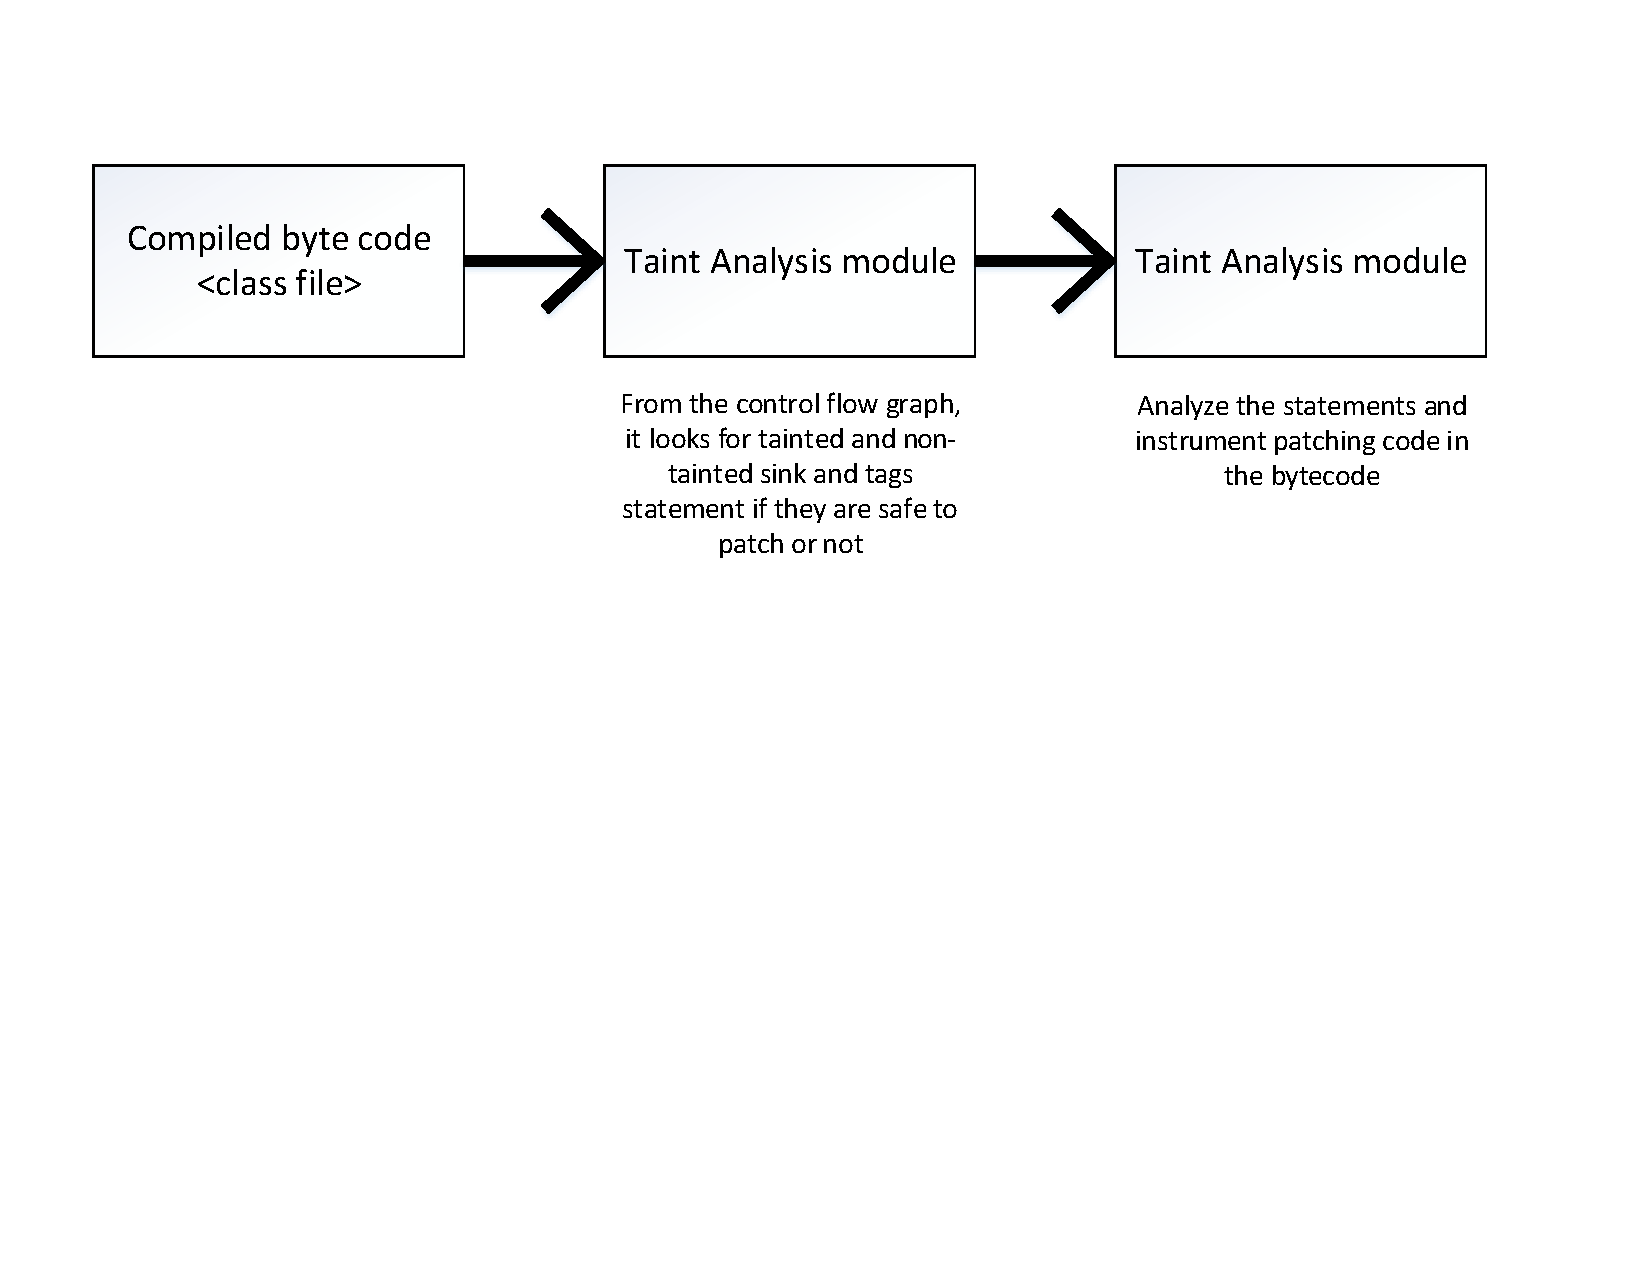
\includegraphics[width=3.0in]{images/OverallDesign.pdf}
\caption{Overall Design}
\label{fig:overallDesign}
\end{figure}

The overall design of the repairing framework is illustrated in
Figure~\ref{fig:overallDesign}. The framework consists of two basic modules.

\begin{enumerate}
  \item \textbf{Taint analysis module :}
  \item \textbf{Repairing Module : }
\end{enumerate}

\section{Benchmark Results}
\label{sec:bench}

\section{Related Work}
\label{sec:rel}

\section{Conclusion and Future Works}
\label{sec:conc}

%\appendix
%\section{Appendix Title}

\acks


% We recommend abbrvnat bibliography style.

\bibliographystyle{abbrvnat}

% The bibliography should be embedded for final submission.
\bibliography{repairbib}


%\begin{thebibliography}{}
%\softraggedright


%\end{thebibliography}

\end{document}

%                       Revision History
%                       -------- -------
%  Date         Person  Ver.    Change
%  ----         ------  ----    ------

%  2013.06.29   TU      0.1--4  comments on permission/copyright notices

